\documentclass[a4paper,onecolumn]{article}
\usepackage[page,toc,titletoc,title]{appendix}
\usepackage{url}
\usepackage{subfigure}
\usepackage[sc]{mathpazo} % Use the Palatino font
\usepackage[T1]{fontenc} % Use 8-bit encoding that has 256 glyphs
\usepackage[utf8]{inputenc} % Use utf-8 as encoding
\linespread{1.05} % Line spacing - Palatino needs more space between lines
\usepackage{microtype} % Slightly tweak font spacing for aesthetics
\usepackage[spanish, activeacute]{babel}
 \decimalpoint
% \usepackage[hmarginratio=1:1,top=32mm,columnsep=20pt]{geometry} % Document marginshttps://www.overleaf.com/project/60211b96f72a79d4c7515e93
% \usepackage[hang, small,labelfont=bf,up,textfont=it,up]{caption} % Custom captions under/above floats in tables or figures
\usepackage{verbatim} % comentarios
\usepackage{listings}
\usepackage{xcolor}
\lstset{
    inputencoding=utf8,
    frame=single,
    basicstyle=\fontsize{8}{11}\selectfont\ttfamily,
    basicstyle=\ttfamily\small,
    keywordstyle=\color{blue}\bfseries,
    identifierstyle=\color{black},
    commentstyle=\color{gray}\itshape,
    stringstyle=\color{red},
    numbers=left,
    numberstyle=\tiny\color{gray},
    stepnumber=1,
    numbersep=10pt,
    showspaces=false,
    showstringspaces=false,
    breaklines=true,
    breakindent=0pt,
    breakatwhitespace=false,
    tabsize=2,
    captionpos=b,
    literate={á}{{\'a}}1
        {ã}{{\~a}}1
        {é}{{\'e}}1
        {ó}{{\'o}}1
        {í}{{\'i}}1
        {ñ}{{\~n}}1
        {¡}{{!`}}1
        {¿}{{?`}}1
        {ú}{{\'u}}1
        {Í}{{\'I}}1
        {Ó}{{\'O}}1
}
\setlength{\parskip}{0.8em}
\usepackage{natbib}
\usepackage{enumitem}
% \setlist[itemize]{noitemsep} % Make itemize lists more compact
% \usepackage{abstract} % Allows abstract customization
% \renewcommand{\abstractnamefont}{\normalfont\bfseries} % Set the "Abstract" text to bold
% \renewcommand{\abstracttextfont}{\normalfont\small\itshape} % Set the abstract itself to small italic text
\usepackage{titlesec}

\usepackage{fancyhdr} % Headers and footers
\pagestyle{fancy} % All pages have headers and footers
\fancyhead{}
\lhead{Hugo Gómez Sabucedo}
\rhead{Minería de datos y modelización predictiva}

\renewcommand{\footrulewidth}{0.2pt}
\usepackage{titling} % Customizing the title section
\usepackage[breaklinks=true]{hyperref} % For hyperlinks in the PDF
%\usepackage{array}
%\newcolumntype{C}[1]{>{\centering\let\newline\\\arraybackslash\hspace{0pt}}m{#1}}
\usepackage{graphicx}
%\usepackage{lipsum} % NO NECESARIO LUEGO
%\usepackage{amsmath}
%\usepackage{wrapfig}
%\usepackage{multicol}
%\usepackage{bm}


\let\stdsection\section
%\renewcommand\section{\newpage\stdsection}

%-------------------------------------------------------------------------------
%	TITLE SECTION
%-------------------------------------------------------------------------------

\setlength{\droptitle}{-4\baselineskip} % Move the title up



\title{\begin{center} \Huge Minería de datos y modelización predictiva \end{center}} % Article title
\author{
    \textsc{\Huge Hugo Gómez Sabucedo} \\ % Your name
    \large \href{mailto:hugogomezsabucedo@gmail.com}{hugogomezsabucedo@gmail.com} \\ [2ex] % Your email address
    \Large \textbf{Máster Big Data, Data Science \& Inteligencia Artificial} \\
    \normalsize Curso 2024-2025 \\
    \large Universidad Complutense de Madrid
}
\date{} % Leave empty to omit a date

\begin{document}
% Print the title
\maketitle
\tableofcontents
\begin{sloppypar}

%-------------------------------------------------------------------------
%	DOCUMENT
%-------------------------------------------------------------------------

\section{Introducción} \label{enunciado}
En esta práctica se nos pide, a partir de un archivo con datos sobre diferentes resultados electorales, seleccionar unas variables, con el objetivo
de construir tanto un modelo de regresión lineal, a partir de una variable objetivo continua; como un modelo de regresión logística, a partir de una
variable binaria. Para ello, se deberán asignar correctamente los tipos de los datos y realizar un análisis de los mismos, con el objetivo inicial 
de depurarlos, para asegurarnos que no tenemos variables incoherentes o que no se ajusten al modelo. A continuación, se corregirán los errores que se 
hayan detectado, así como los valores atípicos y perdidos. Una vez con los datos limpios, podremos analizar las relaciones entre las distintas variables 
input y las variables objetivo, para poder proceder con la creación de los dos modelos solicitados, para cada una de las variables.

Cada registro del archivo viene identificado por Name y CodigoProvincia (ya que, observando el conjunto de datos, se han encontrado municipios con el mismo
nombre pero en provincias diferentes). Adicionalmente, contienen información sobre la CCAA a la que pertenecen. Por otra parte, tenemos las variables objetivo,
que se dividen en las variables continuas (AbstentionPtge, el porcentaje de abstención; IdaPct, el porcentaje de votos a partidos de izquierdas; DchaPct, el
porcentaje de votos a partidos de derechas; y OtrosPct, el porcentaje de votos a otros partidos); y las variables binarias o dicotómicas (AbstencionAlta, que 
vale 1 si el porcentaje de abstención es mayor al 30\% o 0 en otro caso; Izquierda, que toma valor 1 si la suma de votos a los partidos de izquierda es 
superior a la suma de votos a derchas y otros, y 0 en caso contrario; y Derecha, análoga a la anterior, pero para partidos de derechas). De estas, se
escogerá \textbf{AbstentionPtge} para realizar la regresión lineal; e \textbf{Izquierda} para realizar la regresión logística.

Por otra parte, tenemos un conjunto de 29 variables explicativas, las cuales no entraremos a explicar en detalle, pero que se corresponden con aspectos 
demográficos o sociológicos de los distintos municipios, como puede ser el porcentaje de población por tramos de edad, el porcentaje de desempleo por edades 
o sectores, el número de empresas de los municipios por tipo de actividad y la actividad principal del mismo, el porcentaje de población respecto a su CCAA 
y provincia de nacimiento, o, evidentemente, el censo, población, superficie y densidad del municipio.

De esta forma, nuestro objetivo será construir un modelo de regresión lineal para la variable AbstentionPtge y un modelo de regresión logística para la 
variable Izquierda, que nos permitan en el primer caso predecir el porcentaje de abstención, y en el segundo caso, la probabilidad de que los partidos de 
izquierdas sean los más votados.

\section{Importación de datos y análisis descriptivo}
\subsection{Importación}
Para importar los datos, una vez establecido el directorio de trabajo a la carpeta correspondiente con \texttt{os.chdir}, se emplea la siguiente instrucción:
\begin{lstlisting}[language=Python, numbers=none]
    datos = pd.read_excel("DatosElecciones.xlsx", sheet_name='DatosEleccionesEspaña')
\end{lstlisting}

Mediante \texttt{datos.head(5)} podemos ver las 5 primeras filas, y con \texttt{datos.dtypes} podemos ver los tipos de datos de las variables, lo que 
usaremos para comprobar que cada una de las variables tiene asignado el tipo que le corresponde (es decir, numérica o categórica). Creamos una lista con 
las variables, y las dividimos en categóricas y numéricas.
\begin{lstlisting}[language=Python]
    variables = list(datos.columns)
    numericas = datos.select_dtypes(include=['int', 'int32', 'int64','float', 'float32', 'float64']).columns
    categoricas = [v for v in variables if v not in numericas]
\end{lstlisting}
\begin{center}
    \begin{figure}[h!]
        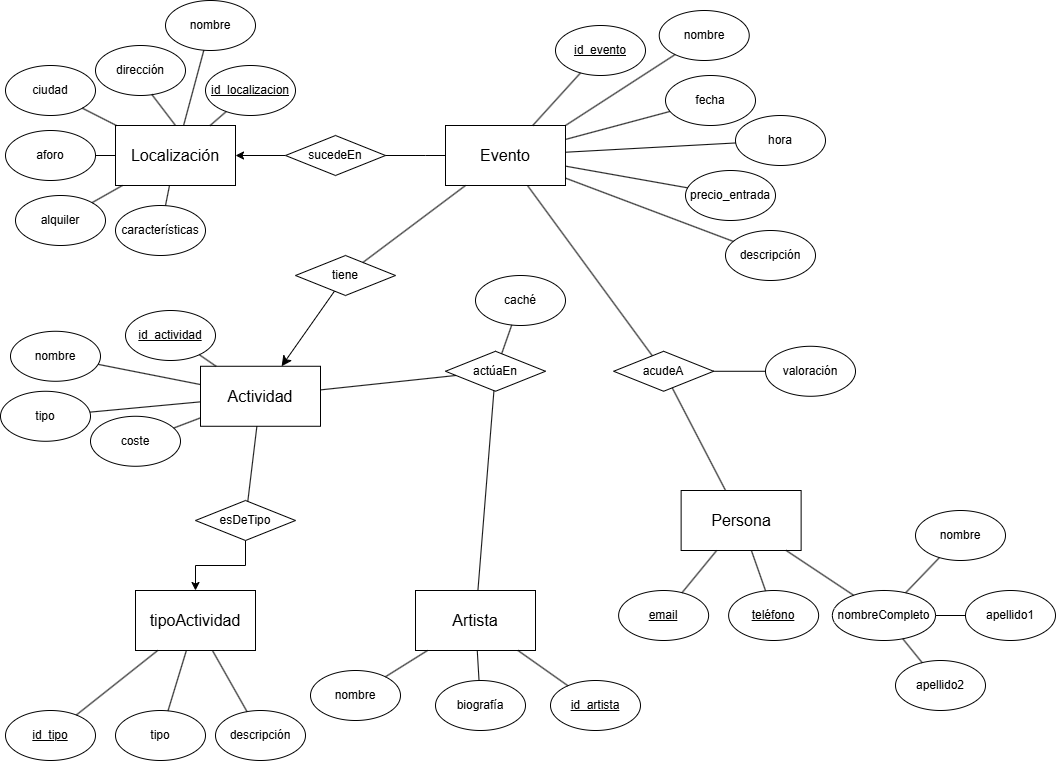
\includegraphics[width=\textwidth]{ejecuciones/MER.png}
    \end{figure}
\end{center}

Puesto que todas las variables están ya correctamente asignadas, podemos pasar directamente al análisis descriptivo de las mismas.

\subsection{Análisis descriptivo}
A continuación haremos el análisis descriptivos de las variables explicativas.

\section{Corrección de errores}

En relación a las variables categóricas, únicamente se realizarán modificaciones en \textit{ActividadPpal}, reagrupando las categorías Construccion e industria
en la categoría Otro, debido a las bajas frecuencias observadas para estas categorías. En la variable \textit{CCAA}, si bien se observa que hay algunas con
más registros que otras, esto forma parte de la naturaleza de los datos, ya que hay algunas comunidades autónomas que tienen más municipios que otras, por lo 
que se ha decidido no realizar ninguna modificación.

\section{Análisis de valores atípicos}
\section{Análisis de valores perdidos}
\section{Detección de relaciones entre variables}
\section{Regresión lineal}
\section{Regresión logística}

\begin{comment}
Todas las variables correcatmente asignadas.
Frecuencia en categoricas. algunos ayuntamieentos repetidos, tiene sentido (mieres en cataluña y asturias).
CCAA:hay mas valores en unas que otras,pero tiene sentido. actividadppal agrupamos construccion e industria en otros. vemos valores perdidos en densidad (?)
abstencion alta, izquierda y derecha dos valores: normal. hay valores perdidos en todos los casos, pero puede deberse a perdidos o a valores repetidos

variables numericas. todas tienen suficientes valores distintos.
poblacion:aplicamos transformacion logaritmica, ya que tienen un rango muy alto debido a municipios que tienen mucha poblacion. lo mismo con censo, inmueble y pob2010.
ageover65pt, foreignerspt tienen valores minimos negativos. deben eliminarse, no es posible. age1965pt, samecomautpt tienen>100. imposible.
explotaciones tiene max 99999. fuera de rango? tratar
tenemos varios nan: totalempresas, industria, construccion, comercttehost, servicios, inmuebles, pob2010, pobchange_pct (estos dos 7 los dos), personasinmueble. tratar

definimos como identificadora NAme y codprovincia

relacion entre valores perdidos: inmuebles y personasinmueble, pob2010 y pobchange, totalcensus y personasinmueble
casi todas las variables tienen valores perdidos. los analizamos. ninguna tiene mas de un 50% (max 9%)
la observacion que mas variables perdidas tiene es un 34por ciento, pero no se elimina (el minimo es 50). pero transformamos la variable a categoricas

datos faltantes en totalEmpresas, industria, construccion, comercttehosteleria, servicios, inmuebles, pob2010, superficie, pobchangeÑ_pct, personasinmueble


relacion entre variables:
v de cramer: xxx
sobre continua: inmuebles, pob2010, servicios, comercttehosteleria, construccion, industria tienen 1.0 de relacion
totalcensus-population y ageu19 vs age0-4 en positivo
unemployu40 vs unemploy25-40, ageover65pct vs age04pt, ageu19pt, age1965pt
pero el objetivo no es eliminar variables porque no queremos hacer un modelo manual

eliminamos industria, construccion, comercttehosteleria, srvicios, inmuebles, pob2010, ageober65, ageunder19 por tener mucha correlacion
eliminamos difcomautpt, samecomautpt, superficie, samecomautdifprovpte, foreignerspt, prop_missing por baja v de cramer 
population, age04 por estar muy relacionada
UnemployMore40_Ptge por lo mismo pero en negativo
personasinmueble presenta tambien gran corealcion
luego se eliminan explotaciones, age1965, servunemploy, agricunemploy, womenpop por tener la menor v de cramer

eliminamos variables en base a: v de cramer <0.1; matriz correlacion: alta; population porque de ella se deriva totalcensus y corr. alta; pct edad por corr alta


mmodelo ganador: stepwise bic
\end{comment}

\appendix
%\section{Anexo: Script de SQL}\label{anexo1}
%\lstinputlisting{HugoGomezSabucedo.sql}

\end{sloppypar}
\end{document}
